\subsection{User Interface}\label{subsubsec:Detailkonzept_UserInterface}

Um die Cocktailmaschine schlussendlich sauber bedienen zu können, wird das in Kapitel \ref{subsec:Hardware_Display} beschriebene Display als Benutzerschnittstelle fungieren. Weitere Schnittstellen werden erstmal nicht verwendet. Damit der Benutzer jedoch die Maschine möglichst intuitiv und einfach bedienen kann, muss zuerst eine geeignete Menustruktur erstellt werden. Im Projekt 5 wird noch nicht die gesamte Struktur auf dem Display programmiert. Trotzdem wird die gesamte Struktur erarbeitet, damit klar ist, welche Schnittstellen benötigt werden. Somit kann ein Testprogramm erstellt werden, welches alle später benötigten Schnittstellen und Funktionen testet. Das komplette Programm wird in Projekt 6 erstellt. Die erarbeitete Menustruktur sieht wie folgt aus.

\subsubsection{Startanzeige}\label{subsubsec:Display_Startanzeige}

Auf der Startanzeige \ref{fig:Display_Startanzeige} kann mit den Pfeiltasten ein gewünschter Cocktail ausgewählt werden. Dabei wird immer ein Bild des Cocktails mit dem dazugehörigen Namen angezeigt. Wird auf den Button «Zutaten» gedrückt erscheint die Zutatenanzeige \ref{fig:Display_Zutatenanzeige}. Wird auf den Button «Menu» gedrückt so gelangt man in die Menuanzeige \ref{fig:Display_Menuanzeige}. Wird auf den Cocktail gedrückt, so gelangt man in die Zubereitungsabfrage \ref{fig:Display_Zubereitungsabfrage}. Mit dem Button «Ohne Alkohol» oder «Mit Alkohol» kann zwischen alkoholischen und nicht alkoholischen Cocktails ausgewählt werden. Wird der Button «Liste» betätigt, so wird die Listenanzeige \ref{fig:Display_Listenanzeige} der alkoholischen oder nicht alkoholischen Cocktails angezeigt.

\begin{figure}[h!]
\centering
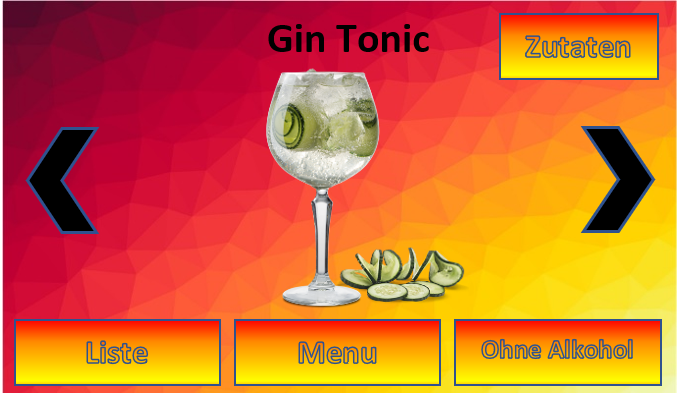
\includegraphics[width=0.7\textwidth]{graphics/Display_Startanzeige.png}
\caption{Ansichtsbild Startanzeige}
\label{fig:Display_Startanzeige}
\end{figure}

\subsubsection{Zutatenanzeige}\label{subsubsec:Display_Zutatenanzeige}

In der Zutatenanzeige \ref{fig:Display_Zutatenanzeige} wird dem Kunden eine Übersicht über die beinhaltenden Zutaten des ausgewählten Cocktails gegeben. Um aus der Zutatenanzeige zu gelangen, kann mit «OK» bestätigt werden.

\begin{figure}[h!]
\centering
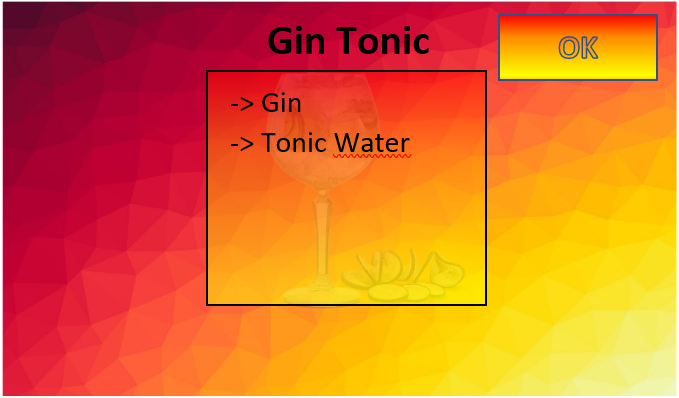
\includegraphics[width=0.7\textwidth]{graphics/Display_Zutatenanzeige.png}
\caption{Ansichtsbild Zutatenanzeige}
\label{fig:Display_Zutatenanzeige}
\end{figure}

\subsubsection{Listenanzeige}\label{subsubsec:Display_Listenanzeige}

In der Listenanzeige \ref{fig:Display_Listenanzeige} wird dem Kunden eine Liste der verfügbaren Cocktails aufgezeigt, wobei dieser mit den Pfeiltasten durchblättern und den gewünschten Cocktail auswählen kann. Wird auf einen Cocktail gedrückt, so gelangt man wieder in die Startanzeige \ref{fig:Display_Startanzeige} mit dem ausgewählten Cocktail.

\begin{figure}[h!]
\centering
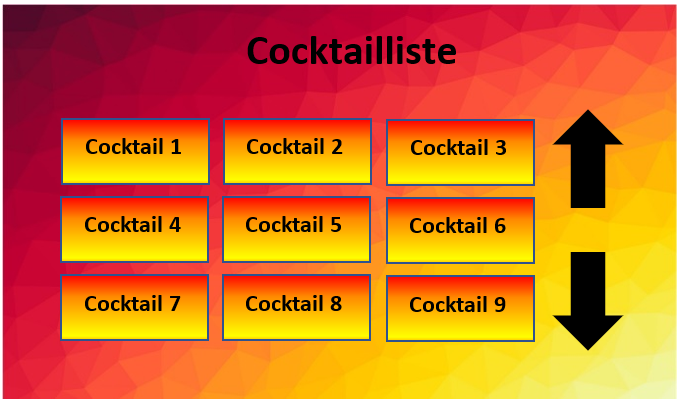
\includegraphics[width=0.7\textwidth]{graphics/Display_Listenanzeige.png}
\caption{Ansichtsbild Listenanzeige}
\label{fig:Display_Listenanzeige}
\end{figure}

\subsubsection{Zubereitungsabfrage}\label{subsubsec:Display_Zubereitungsabfrage}

In der Zubereitungsabfrage \ref{fig:Display_Zubereitungsabfrage} wird der Kunde gefragt, ob er einen 3dl oder 5dl Cocktail zubereiten will. Wird «Ja 3dl» betätigt, so wird ein 3dl Getränk zubereitet. Wird «Ja 5dl» betätigt, so wird ein 5dl Getränk zubereitet und man gelangt auf den Zubereitungsbildschirm \ref{fig:Display_Zubereitungsbildschirm}. Mit «Abbrechen» gelangt man zurück zur Startanzeige \ref{fig:Display_Startanzeige}.

\begin{figure}[h!]
\centering
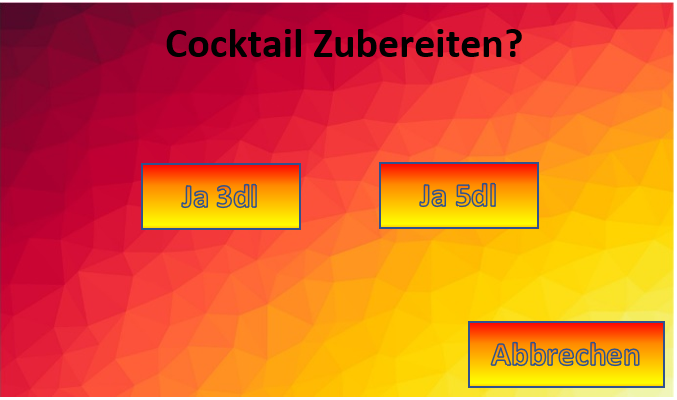
\includegraphics[width=0.7\textwidth]{graphics/Display_Zubereitungsabfrage.png}
\caption{Ansichtsbild Zubereitungsabfrage}
\label{fig:Display_Zubereitungsabfrage}
\end{figure}

\subsubsection{Zubereitungsbildschirm}\label{subsubsec:Display_Zubereitungsbildschirm}

Auf dem Zubereitungsbildschirm \ref{fig:Display_Zubereitungsbildschirm} wird der Kunde darüber informiert, dass der Cocktail zubereitet wird. Gleichzeitig wird dem Kunden ein Fact zum gewählten Cocktail gezeigt, um die Wartezeit ein wenig zu versüssen. Mit dem Button «Abbrechen» kann der laufende Prozess abgebrochen werden und es erscheint die Abbruchanzeige \ref{fig:Display_Abbruchanzeige}. Ist der Cocktail fertig, so wird dem Kunden die Bereitanzeige \ref{fig:Display_Bereitanzeige} angezeigt. 

\begin{figure}[h!]
\centering
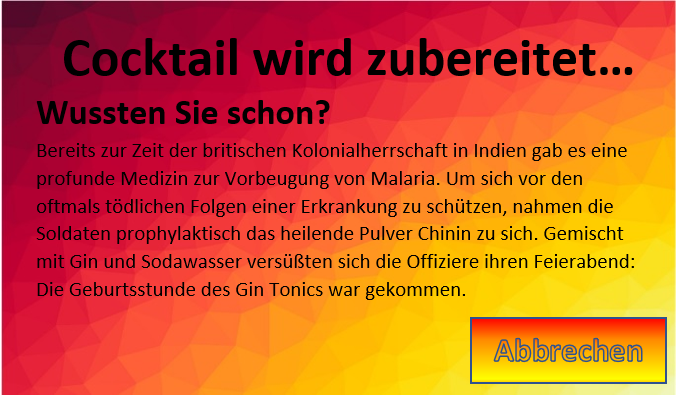
\includegraphics[width=0.7\textwidth]{graphics/Display_Zubereitungsbildschirm.png}
\caption{Ansichtsbild Zubereitungsbildschirm}
\label{fig:Display_Zubereitungsbildschirm}
\end{figure}

\subsubsection{Bereitanzeige}\label{subsubsec:Display_Bereitanzeige}

Die Bereitanzeige \ref{fig:Display_Bereitanzeige} zeigt dem Kunden, dass der Cocktail fertig ist und dieser nun entnommen werden kann. Dieser Bildschirm erscheint für 5 Sekunden. Nach dieser Zeit erscheint automatisch wieder die Startanzeige \ref{fig:Display_Startanzeige}.

\begin{figure}[h!]
\centering

\includegraphics[width=0.7\textwidth]{graphics/Display_Bereitanzeige.png}
\caption{Ansichtsbild Bereitanzeige}
\label{fig:Display_Bereitanzeige}
\end{figure}

\subsubsection{Menuanzeige}\label{subsubsec:Display_Menuanzeige}

Wird in der Menuanzeige \ref{fig:Display_Menuanzeige} «Cocktail bearbeiten» ausgewählt, so kommt man in die Bearbeitungsanzeige \ref{fig:Display_Bearbeitungsanzeige}. Wird «Maschine Reinigen» gedrückt, so gelangt man in die Reinigungsanzeige1 \ref{fig:Display_Reinigungsanzeige1}. Wird «Maschineninfo» betätigt, so gelangt man in die Infoanzeige \ref{fig:Display_Infoanzeige}. Mit «Zurück» gelangt man wieder auf den Startanzeige \ref{fig:Display_Startanzeige}.

\begin{figure}[h!]
\centering
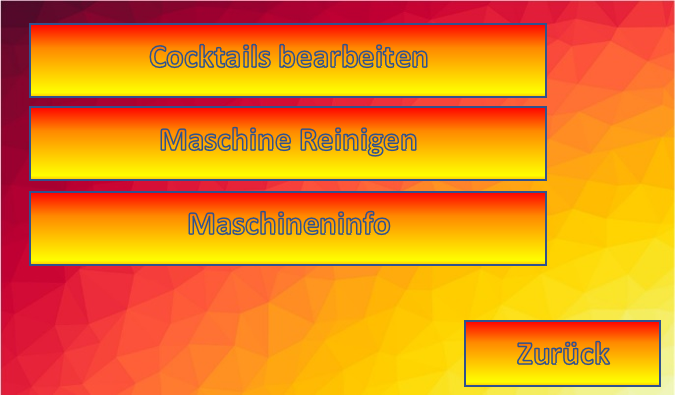
\includegraphics[width=0.7\textwidth]{graphics/Display_Menuanzeige.png}
\caption{Ansichtsbild Menuanzeige}
\label{fig:Display_Menuanzeige}
\end{figure}

\subsubsection{Bearbeitungsanzeige}\label{subsubsec:Display_Bearbeitungsanzeige}

In der Bearbeitungsanzeige \ref{fig:Display_Bearbeitungsanzeige} kann der zu bearbeitende Cocktail ausgewählt werden. Wird einer ausgewählt, so gelangt man in die dazugehörige Cocktaileinstellungsanzeige \ref{fig:Display_Cocktaileinstellungsanzeige}. Mit den Pfeiltasten kann zwischen den verschiedenen Cocktails navigiert werden. Wird «Zurück» betätigt, so gelangt man wieder zur Menuanzeige \ref{fig:Display_Menuanzeige}. 

\begin{figure}[h!]
\centering
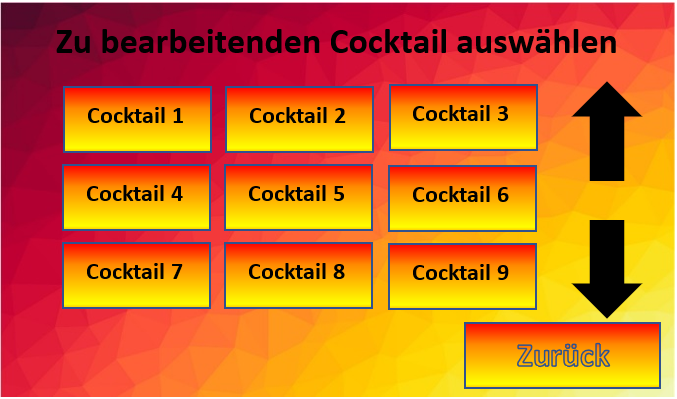
\includegraphics[width=0.7\textwidth]{graphics/Display_Bearbeitungsanzeige.png}
\caption{Ansichtsbild Bearbeitungsanzeige}
\label{fig:Display_Bearbeitungsanzeige}
\end{figure}

\subsubsection{Cocktaileinstellungsanzeige}\label{subsubsec:Display_Cocktaileinstellungsanzeige}

In der Cocktaileinstellungsanzeige \ref{fig:Display_Cocktaileinstellungsanzeige} kann mittels Schieberegler jede Zutat in der Menge angepasst werden. Es kann jedoch nie 100\% überschritten werden. Wird «Standarteinstellung» gedrückt, so wird der Cocktail auf die jeweilige Standarteinstellung eingestellt. Betätigt man «OK», so gelangt man wieder in die Bearbeitungsanzeige \ref{fig:Display_Bearbeitungsanzeige}.

\begin{figure}[h!]
\centering
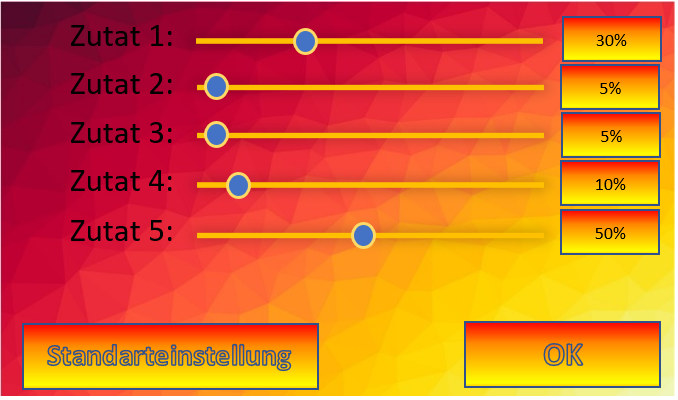
\includegraphics[width=0.7\textwidth]{graphics/Display_Cocktaileinstellungsanzeige.png}
\caption{Ansichtsbild Cocktaileinstellungsanzeige}
\label{fig:Display_Cocktaileinstellungsanzeige}
\end{figure}

\subsubsection{Reinigungsanzeige1}\label{subsubsec:Display_Reinigungsanzeige1}

In der Reinigungsanzeige1 \ref{fig:Display_Reinigungsanzeige1} wird man Stück für Stück durch den Reinigungsmodus geführt. In der Reinigungsanzeige1 wird man aufgefordert den Reinigungsbehälter mit warmem Wasser zu befüllen und alle Schläuche darin ein zu setzen. Wird «Weiter» gedrückt, so gelangt man in die Reinigungsanzeige2 \ref{fig:Display_Reinigungsanzeige2}. Wird «Abbrechen» gedrückt, so gelangt man zurück in die Menuanzeige \ref{fig:Display_Menuanzeige}.

\begin{figure}[h!]
\centering
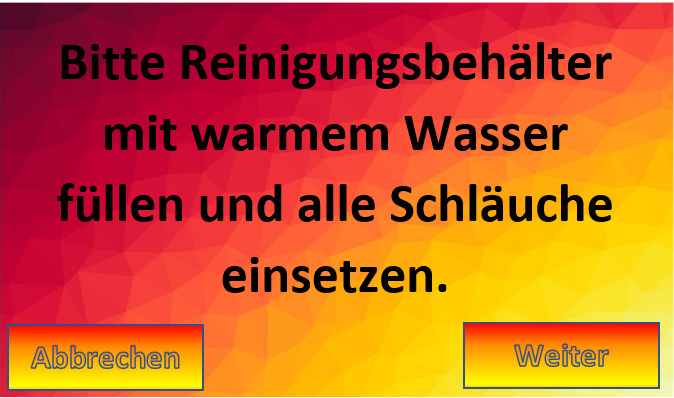
\includegraphics[width=0.7\textwidth]{graphics/Display_Reinigungsanzeige1.png}
\caption{Ansichtsbild Reinigungsanzeige1}
\label{fig:Display_Reinigungsanzeige1}
\end{figure}

\subsubsection{Reinigungsanzeige2}\label{subsubsec:Display_Reinigungsanzeige2}

In der Reinigungsanzeige2 \ref{fig:Display_Reinigungsanzeige2} wird gefragt, ob der Reinigungsvorgang gestartet werden soll. Mit «Start» wird der Vorgang gestartet und man gelangt in die Reinigungsanzeige3 \ref{fig:Display_Reinigungsanzeige3}. Wird «Abbrechen» gedrückt, so gelangt man in die Menuanzeige \ref{fig:Display_Menuanzeige} zurück.

\begin{figure}[h!]
\centering
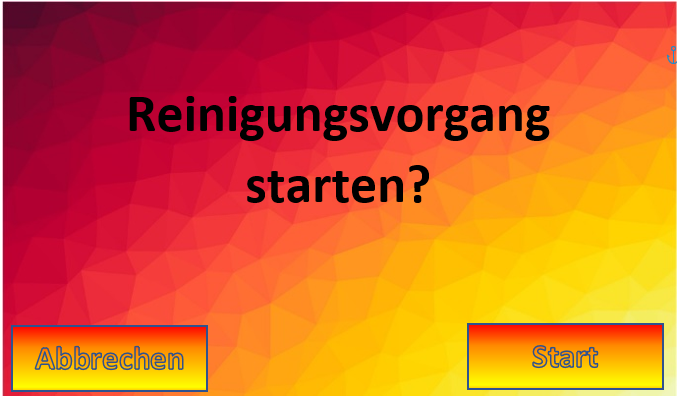
\includegraphics[width=0.7\textwidth]{graphics/Display_Reinigungsanzeige2.png}
\caption{Ansichtsbild Reinigungsanzeige2}
\label{fig:Display_Reinigungsanzeige2}
\end{figure}

\subsubsection{Reinigungsanzeige3}\label{subsubsec:Display_Reinigungsanzeige3}

In der Reinigungsanzeige3 \ref{fig:Display_Reinigungsanzeige3} wird der Kunde darüber informiert, dass die Reinigung nun durchgeführt wird. Die Reinigung kann zu diesem Zeitpunkt nicht abgebrochen werden, da sonst Flüssigkeit in den Schläuchen verbleiben könnte, welche den nächsten Cocktail ungeniessbar macht. Ist die Reinigung beendet, so erscheint die Startanzeige \ref{fig:Display_Startanzeige}.

\begin{figure}[h!]
\centering
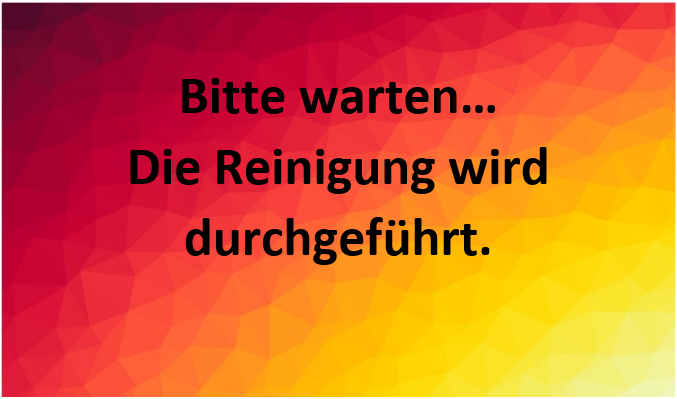
\includegraphics[width=0.7\textwidth]{graphics/Display_Reinigungsanzeige3.png}
\caption{Ansichtsbild Reinigungsanzeige3}
\label{fig:Display_Reinigungsanzeige3}
\end{figure}

\newpage

\subsubsection{Infoanzeige}\label{subsubsec:Display_Infoanzeige}

In der Infoanzeige \ref{fig:Display_Infoanzeige} werden dem Kunden Informationen zur Cocktailsmaschine gegeben. Mit «Zurück» gelangt man erneut in die Menuanzeige \ref{fig:Display_Menuanzeige}.

\begin{figure}[h!]
\centering
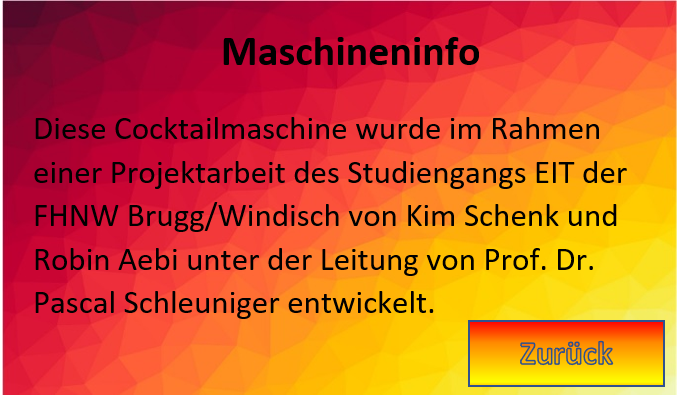
\includegraphics[width=0.7\textwidth]{graphics/Display_Infoanzeige.png}
\caption{Ansichtsbild Infoanzeige}
\label{fig:Display_Infoanzeige}
\end{figure}

\subsubsection{Abbruchanzeige}\label{subsubsec:Display_Abbruchanzeige}

Wird ein Vorbereitungsvorgang abgebrochen, so erscheint die Abbruchanzeige \ref{fig:Display_Abbruchanzeige}, welcher den Kunden darüber informiert, dass der Vorgang abgebrochen wurde. Sobald der Abbruchvorgang beendet ist, erscheint wieder die Startanzeige \ref{fig:Display_Startanzeige}.

\begin{figure}[h!]
\centering
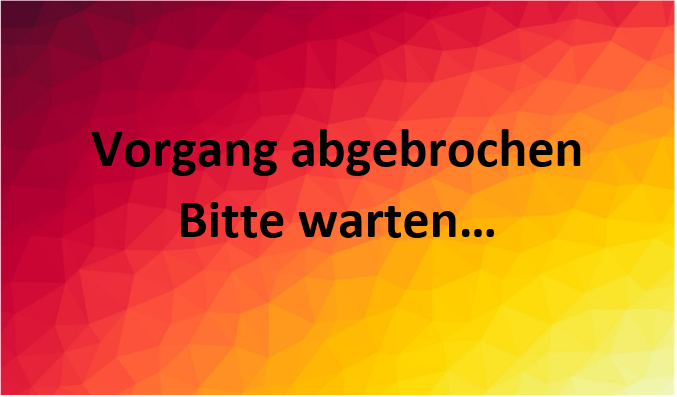
\includegraphics[width=0.7\textwidth]{graphics/Display_Abbruchanzeige.png}
\caption{Ansichtsbild Abbruchanzeige}
\label{fig:Display_Abbruchanzeige}
\end{figure}

\newpage

\subsubsection{Fehleranzeige}\label{subsubsec:Display_Fehleranzeige}

Wird über eine gewisse Zeit trotz eingeschalteter Pumpen kein Durchfluss festgestellt, so erscheint die Fehleranzeige \ref{fig:Display_Fehleranzeige} und die Maschine stoppt. Der Benutzer wird dabei aufgefordert die Flüssigkeitsbehälter zu kontrollieren und diese gegebenenfalls wieder aufzufüllen. Ist dies erledigt, so kann mit «Erledigt» bestätigt werden und der Cocktail wird an der gestoppten Stelle fortgesetzt mit dem vorherigen Zubereitungsbildschirm \ref{fig:Display_Zubereitungsbildschirm}.

\begin{figure}[h!]
\centering

\includegraphics[width=0.7\textwidth]{graphics/Display_Fehleranzeige.png}
\caption{Ansichtsbild Fehleranzeige}
\label{fig:Display_Fehleranzeige}
\end{figure}